\documentclass[10pt,twocolumn]{article}
\usepackage[a4paper,margin=1.55cm,columnsep=0.55cm]{geometry}
\usepackage[T1]{fontenc}
\usepackage[utf8]{inputenc}
\usepackage{lmodern}
\usepackage{microtype}
\usepackage{amsmath,amssymb,amsthm}
\usepackage{booktabs}
\usepackage{graphicx}
\usepackage{xcolor}
\usepackage{xurl}
\usepackage{hyperref}
\usepackage{enumitem}
\usepackage[most]{tcolorbox}
\usepackage{balance}

\definecolor{minblue}{HTML}{124E78}
\definecolor{minorange}{HTML}{F28C28}
\definecolor{taskyellow}{HTML}{FFF4CC}
\hypersetup{colorlinks=true,linkcolor=minblue,citecolor=minblue,urlcolor=minblue}
\setlength{\parindent}{1em}
\setlength{\parskip}{0.2em}
\setlist{nosep,leftmargin=*}
\newtheorem{definition}{Definition}
\newtheorem{proposition}{Proposition}
\newtheorem{lemma}{Lemma}

\IfFileExists{generated_macros.tex}{% Auto-generated by scripts/run_experiments.py; do not edit.
\newcommand{\ScenarioCount}{360}
\newcommand{\ExperimentRuns}{1,800}
\newcommand{\MinAttackPrevention}{100.0\%}
\newcommand{\MinBlockedVolume}{14.4\%}
\newcommand{\MinAvailability}{85.6\%}
\newcommand{\MinRecovery}{81.2\%}
\newcommand{\GlobalBlockedVolume}{100.0\%}
\newcommand{\GlobalRecovery}{2.5\%}
\newcommand{\ManualAttackPrevention}{91.7\%}
\newcommand{\MinPolicySize}{1.34}
\newcommand{\AvailabilityGain}{85.6\%}
}{
  \newcommand{\ScenarioCount}{360}
  \newcommand{\ExperimentRuns}{1,800}
  \newcommand{\MinAttackPrevention}{100.0\%}
  \newcommand{\MinBlockedVolume}{14.4\%}
  \newcommand{\MinAvailability}{85.6\%}
  \newcommand{\MinRecovery}{81.2\%}
  \newcommand{\GlobalBlockedVolume}{100.0\%}
  \newcommand{\GlobalRecovery}{2.5\%}
  \newcommand{\ManualAttackPrevention}{91.7\%}
  \newcommand{\MinPolicySize}{1.34}
  \newcommand{\AvailabilityGain}{85.6\%}
}

\newtcolorbox{mehrantask}[1]{
  colback=taskyellow,colframe=minorange,fonttitle=\bfseries,
  title={Mathematical completion required: #1},breakable
}

\title{\textbf{MinPause: Recovery-Preserving Emergency Control for DeFi Lending}}
\author{Niko Rokni\\\small Draft for mathematical completion and conference submission}
\date{November 2026}

\begin{document}
\raggedbottom
\maketitle

\begin{abstract}
Emergency pauses can stop non-atomic decentralized-finance attacks, but a global freeze also blocks legitimate activity and may prevent borrowers from repaying debt or adding collateral.  We formulate emergency response as a constrained, weighted hitting-set problem: select the least-cost set of protocol operations whose suspension intersects every identified attack path while designated recovery operations remain available.  We implement \emph{MinPause}, an exact and auditable policy synthesizer for the small operation sets exposed by lending markets, and evaluate it against no intervention, a global freeze, a coarse risk pause, and a manual selective policy.  A deterministic Latin-hypercube design covers \ScenarioCount{} market and incident configurations, producing \ExperimentRuns{} policy evaluations.  MinPause blocks \MinAttackPrevention{} of modelled attack paths while retaining \MinAvailability{} of legitimate activity and keeping repayment and collateral top-up available.  The mean policy contains only \MinPolicySize{} paused operations, compared with nine under a global freeze.  The artifact includes source code, tests, scenario-level results, and manuscript-generation scripts.  Formal security, feasibility, recovery, and complexity claims are stated precisely but their final proofs are isolated and explicitly assigned for mathematical completion before submission.
\end{abstract}

\section{Introduction}
Decentralized lending protocols operate continuously, settle transactions quickly, and expose composable entry points to untrusted callers.  When an incident is detected, a guardian can often pause a protocol faster than a governance upgrade can be proposed, audited, and executed.  This response can be effective when an attack is non-atomic: Zhou et al. found that 56\% of the attacks in their incident corpus left a potential rescue interval \cite{zhou2023sok}.  Yet pausing is not free.  A global freeze exchanges integrity for availability and can prevent users from reducing their own exposure.  In a lending market, blocking \texttt{repay} or collateral top-up during a price shock may turn a containable incident into avoidable liquidation or bad debt.

Production systems therefore expose controls at different granularities.  OpenZeppelin's \texttt{Pausable} pattern guards selected state-changing operations \cite{openzeppelin2023ir,openzeppelin2026pausable}; Compound-style guardians can suspend individual actions, and recent incident-response guidance distinguishes broad, function-level, and asset-level stops \cite{owasp2026circuit}.  However, the policy determining \emph{which} functions to stop is commonly written by hand.  A manual policy may be too broad, leaving unnecessary denial of service, or too narrow, leaving an alternative attack path executable.

This paper asks: \emph{Given a set of plausible attack paths, which minimum-cost operations should be paused so that every path is interrupted while borrower recovery remains possible?}  We answer with MinPause, a transparent policy synthesizer built around an action--effect graph and a binary optimization problem.  Recovery-critical actions are hard constraints rather than soft preferences.  If an identified path can only be interrupted by disabling a recovery-critical action, the model reports infeasibility instead of silently weakening the requirement.

The contributions are:
\begin{itemize}
  \item a protocol-independent action--effect representation of lending operations, state effects, and alternative attack paths;
  \item the Minimum Recovery-Preserving Pause problem, combining path coverage, legitimate-use cost, and group-level disruption;
  \item an exact, deterministic solver and a public experimental artifact with \ScenarioCount{} reproducible scenarios;
  \item a counterfactual comparison of four conventional responses with MinPause using security, availability, recovery, bad-debt, and distributional metrics; and
  \item four explicit theoretical claims, separated into a mathematical completion section so that assumptions and proofs can be independently checked before submission.
\end{itemize}

\section{Related Work}
\subsection{DeFi incidents and response}
The DeFi security literature has catalogued smart-contract, economic, oracle, governance, and composability failures.  The SoK by Zhou et al. combines 181 incidents with academic and audit evidence, studies rescue intervals, and measures the use and timing of emergency pauses \cite{zhou2023sok}.  Daian et al. show how transaction ordering and miner-extractable value create adversarial execution environments \cite{daian2020flash}.  Qin et al. empirically document liquidation design and borrower costs across major lending protocols \cite{qin2021liquidations}.  These studies motivate rapid containment, but do not synthesize the scope of the containment action.

Emergency intervention also has economic effects.  During the Ethereum Merge, Aave paused ETH borrowing while Compound altered interest parameters and borrowing caps.  Heimbach et al. show that these interventions affected liquidity and redistributed hard-fork-arbitrage value \cite{heimbach2023merge}.  More generally, rigid lending terms can amplify fragility and multiple-equilibrium behaviour \cite{chiu2025fragility}.  MinPause focuses on the narrower operational question that precedes such welfare analysis: which actions must be disabled after an alert?

\subsection{Circuit breakers and formal models}
Industry guidance recommends monitoring, pause roles, function limits, rate limits, and rehearsed recovery procedures \cite{openzeppelin2023ir,owasp2026recovery}.  OpenZeppelin notes that a pause can be broad or granular and that a broad pause creates a denial-of-service state for legitimate users \cite{openzeppelin2023ir}.  Formal work has represented the circuit-breaker design pattern with Dynamic Condition Response graphs, providing an unambiguous behavioural specification \cite{eshghie2026dcr}.  That work models how a pause behaves; MinPause instead chooses a pause set from competing security and availability requirements.

The closest combinatorial abstraction is weighted hitting set: every attack path is a set, and a feasible pause policy must intersect every such set.  Hitting-set formulations are well understood \cite{vazirani2001approximation}, but their use with hard recovery constraints and borrower-level counterfactual evaluation is, to our knowledge, absent from the DeFi pause literature.  This novelty claim is intentionally narrow: MinPause does not claim to invent pausing, attack graphs, or hitting set individually.

\section{System and Threat Model}
\subsection{Protocol state}
Let $F$ be the finite set of independently pausable operations.  Our reference market uses
\begin{align*}
F=\{&\textsf{supply},\textsf{withdraw},\textsf{borrow},\textsf{repay},
\textsf{addCollateral},\\
&\textsf{liquidate},\textsf{flashLoan},\textsf{swap},\textsf{oracleUpdate}\}.
\end{align*}
The abstraction is not tied to a particular implementation: an operation can represent one Solidity entry point, several entry points sharing a pause flag, or an external adapter that governance can isolate.

Borrower $i$ has post-shock state
\[
s_i(t)=\big(C_i(t),D_i(t),\ell_i,A_i^D,A_i^C,g_i\big),
\]
where $C_i$ and $D_i$ are collateral and debt values, $\ell_i$ is the liquidation threshold, $A_i^D$ is immediately repayable debt, $A_i^C$ is available additional collateral, and $g_i$ is a user-size group.  The health factor is
\begin{equation}
H_i(t)=\frac{\ell_i C_i(t)}{D_i(t)}.
\label{eq:hf}
\end{equation}
A position is at risk when $H_i<1$.

\subsection{Attack paths and responder}
An attack path $P_k\subseteq F$ is the set of operations required by one executable route to a prohibited economic effect.  Multiple paths may reach the same effect.  The detector supplies a family $\mathcal P=\{P_1,\ldots,P_m\}$; path extraction itself is outside the present scope.  The responder controls operation-level pause flags but cannot reverse settled transactions, change historical oracle observations, or stop calls that finish atomically before detection.

We assume the guardian is not compromised, pause transactions are eventually included, and the abstract paths are sound for the incident under study.  These are strong assumptions and are tested only through sensitivity analysis, not formally guaranteed by the implementation.

\section{MinPause Framework}
\subsection{Decision variables and constraints}
For each $f\in F$, let
\[
x_f=\begin{cases}1,&f\text{ is paused},\\0,&f\text{ remains active}.
\end{cases}
\]
Every identified path must contain a paused operation:
\begin{equation}
\sum_{f\in P_k}x_f\geq1,\qquad k=1,\ldots,m.
\label{eq:cover}
\end{equation}
Let $R\subseteq F$ be the recovery-critical set.  In the implementation,
$R=\{\textsf{repay},\textsf{addCollateral}\}$, and
\begin{equation}
x_r=0,\qquad r\in R.
\label{eq:recovery}
\end{equation}

Each operation has normalized legitimate-use cost $c_f\geq0$.  Group-specific costs $c_{fg}$ represent the share borne by group $g$.  For a policy $x$, group burden is
\[
B_g(x)=\frac{\sum_f c_{fg}x_f}{\sum_f c_{fg}},
\]
and disparity is $\Delta(x)=\max_gB_g(x)-\min_gB_g(x)$.  MinPause solves
\begin{equation}
\min_{x\in\{0,1\}^{|F|}}
\sum_{f\in F}c_fx_f+\lambda\Delta(x)
\quad\text{s.t. \eqref{eq:cover}--\eqref{eq:recovery}.}
\label{eq:objective}
\end{equation}
We use $\lambda=0.15$ in the main experiment.  The fairness term is a design choice, not a claim that the three size groups capture all meaningful welfare differences.

\subsection{Exact synthesis algorithm}
Because a market normally exposes only a small number of independent pause flags, the reference implementation enumerates all subsets of $F\setminus R$.  For each subset it checks path coverage, computes the objective, and retains the minimum with deterministic tie-breaking by cardinality and operation name.  With nine operations and two protected recovery operations, at most $2^7=128$ subsets are evaluated per incident.  This exact implementation is easier to audit than a heuristic and removes solver-specific variability.

The output contains the paused set, feasibility flag, legitimate-use cost, disparity, and objective value.  An infeasible result is operationally meaningful: the identified threat cannot be contained under the declared recovery guarantee, so the responder must relax the guarantee, upgrade, migrate, or use a broader emergency procedure.

\begin{figure}[t]
  \centering
  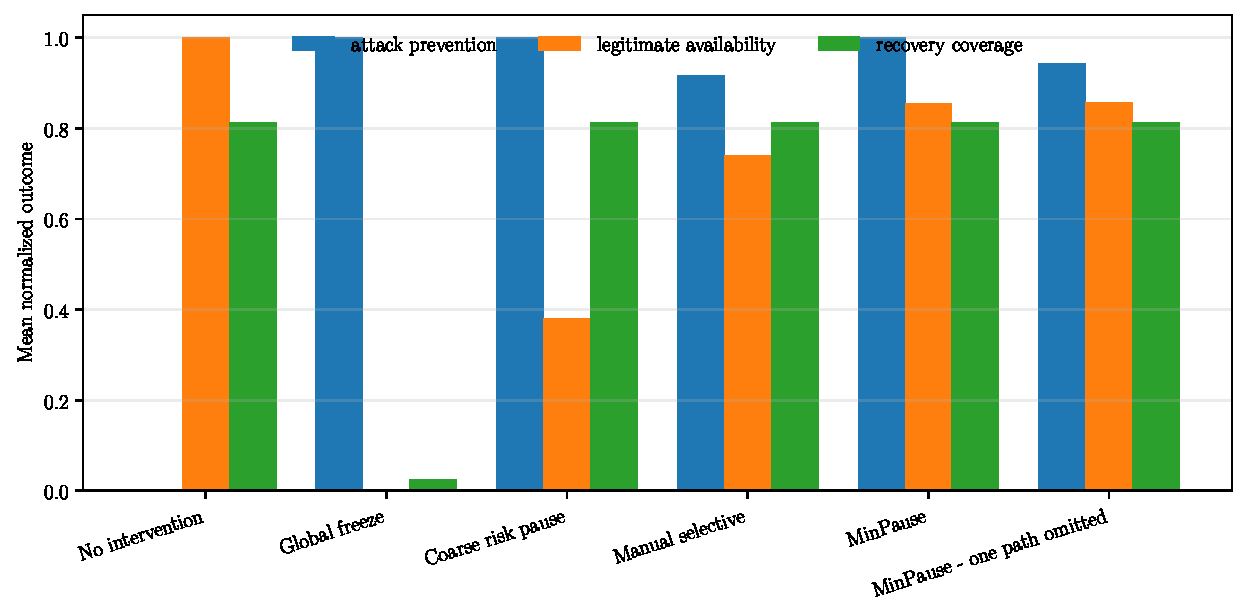
\includegraphics[width=\columnwidth]{../figures/policy_comparison.pdf}
  \caption{Mean security, availability, and borrower-recovery outcomes across \ScenarioCount{} scenarios.}
  \label{fig:comparison}
\end{figure}

\section{Mathematical Analysis: Completion Required}
This section contains the only unresolved material in the manuscript.  The computational method and empirical results do not assume that the following proofs have already been established.  Each statement must be checked, corrected if necessary, and proved before submission.

\begin{mehrantask}{M1---Attack-path coverage}
\textbf{Information supplied.}  Let the protocol abstraction be a directed state-transition system.  Each prohibited execution trace is mapped to an operation set $P_k$.  A pause policy removes every transition labelled by an operation in $X=\{f:x_f=1\}$.

\textbf{Proposed statement.}  If $X\cap P_k\neq\varnothing$ for every $P_k\in\mathcal P$, then no trace represented by $\mathcal P$ remains executable in the paused transition system.

\textbf{To complete.}  Define precisely the mapping from ordered traces to operation sets; state the soundness assumption needed to avoid loss of order/multiplicity information; provide a short proof, or replace the set abstraction with an ordered-path formulation if the statement is not valid as written.
\end{mehrantask}

\begin{mehrantask}{M2---Feasibility characterization}
\textbf{Candidate condition.}
\begin{equation}
\forall P_k\in\mathcal P,\qquad P_k\setminus R\neq\varnothing.
\label{eq:feasible-condition}
\end{equation}
\textbf{Proposed statement.}  With no additional restrictions on pausing operations in $F\setminus R$, problem \eqref{eq:objective} is feasible if and only if \eqref{eq:feasible-condition} holds.

\textbf{To complete.}  Verify both directions, state whether empty paths or unavailable pause flags require exclusions, and supply a formal proof.
\end{mehrantask}

\begin{mehrantask}{M3---Finite borrower recovery}
From \eqref{eq:hf}, repayment $a_D$ and additional collateral $a_C$ give
\[
H_i'=\frac{\ell_i(C_i+a_C)}{D_i-a_D},
\quad 0\leq a_D<D_i,\quad a_C\geq0.
\]
Both actions are monotone in the expected direction when prices and $\ell_i$ are fixed.

\textbf{To complete.}  State necessary and sufficient resource conditions for the existence of admissible $(a_D,a_C)$ such that $H_i'\geq1$; prove monotonicity and finite reachability under explicit assumptions; distinguish ``the recovery operation is callable'' from ``the borrower has sufficient resources to recover.''  The empirical metric uses the latter distinction and never assumes universal recovery.
\end{mehrantask}

\begin{mehrantask}{M4---Computational complexity}
\textbf{Proposed statement.}  The decision form of MinPause with $R=\varnothing$ and $\lambda=0$ is NP-complete; the optimization form is NP-hard by reduction from weighted hitting set.

\textbf{To complete.}  Give a clean polynomial reduction, define the decision threshold, establish membership in NP, and explain that the deployed exact solver remains practical because $|F|$ is small.  Do not claim polynomial-time optimality for arbitrary protocol size.
\end{mehrantask}

\section{Experimental Methodology}
\subsection{Design and reproducibility}
We generate \ScenarioCount{} configurations using a seeded, jittered Latin hypercube.  The sampled dimensions are collateral price shock $[0.02,0.45]$, utilization $[0.35,0.98]$, detection delay $[1,90]$ minutes, potential attack loss $[0.25,20]$ million USD on a logarithmic scale, liquidity $[1,100]$ million USD on a logarithmic scale, borrower count $[120,600]$, recovery capacity $[0.04,0.50]$, activity skew, and incident family.  Four incident families---oracle, liquidity, accounting, and composite---contain three to five alternative attack paths.

Borrower debt is lognormally distributed, initial health factors lie in $[1.03,1.85]$, and liquidation thresholds lie in $[0.72,0.86]$.  A price shock is applied before policy evaluation.  Available repayment and collateral top-up are sampled as bounded shares of each position.  These synthetic distributions create controlled counterfactuals; they are not estimates of a named production market.

Every scenario is evaluated under five policies:
\begin{enumerate}
  \item \textbf{No intervention}: all operations remain active;
  \item \textbf{Global freeze}: all nine operations are disabled;
  \item \textbf{Coarse risk pause}: withdraw, borrow, liquidate, flash loan, and swap are disabled;
  \item \textbf{Manual selective}: borrow, flash loan, and oracle update are disabled; and
  \item \textbf{MinPause}: the solution of \eqref{eq:objective}.
\end{enumerate}
The complete design yields \ExperimentRuns{} policy--scenario evaluations.  The repository stores scenario-level CSV output, aggregate summaries, figures, fixed seeds, and automated tests.

\subsection{Metrics}
Attack prevention is the fraction of identified paths intersected by the pause set.  Detection delay determines the preventable share of potential loss through $e^{-\tau/55}$; this reduced-form decay is used consistently across policies and is varied through $\tau$.  Legitimate availability is one minus the normalized pause cost.  Recovery coverage is the share of post-shock at-risk borrowers able to reach $H_i\geq1$ using whichever of repayment and collateral top-up remain callable, subject to their sampled resource limits.  We also report policy cardinality, bad-debt proxy, liquidation count, deferred risky positions, and group-burden disparity.

\section{Results}
\begin{table*}[t]
\centering
\caption{Mean results across \ScenarioCount{} scenarios. Higher is better for attack prevention, availability, and recovery; lower is better for policy size and disparity.}
\label{tab:main-results}
\begin{tabular}{lrrrrr}
\toprule
Policy & Attack prevention & Availability & Recovery coverage & Policy size & Disparity \\
\midrule
No intervention & 0.0\% & 100.0\% & 81.2\% & 0.00 & 0.000 \\
Global freeze & 100.0\% & 0.0\% & 2.5\% & 9.00 & 0.000 \\
Coarse risk pause & 100.0\% & 38.0\% & 81.2\% & 5.00 & 0.334 \\
Manual selective & 91.7\% & 74.0\% & 81.2\% & 3.00 & 0.058 \\
\textbf{MinPause} & \textbf{100.0\%} & \textbf{85.6\%} & \textbf{81.2\%} & \textbf{1.34} & \textbf{0.042} \\
\bottomrule
\end{tabular}
\end{table*}

\subsection{Security and availability}
Table~\ref{tab:main-results} and Fig.~\ref{fig:comparison} show the central trade-off.  Global freeze and coarse risk pause cover every modelled path, but retain 0.0\% and 38.0\% of legitimate activity, respectively.  The fixed manual policy retains 74.0\% availability but covers only \ManualAttackPrevention{} of paths.  MinPause covers \MinAttackPrevention{} while pausing only \MinBlockedVolume{} of normalized legitimate activity.  Its mean policy size is \MinPolicySize{} operations.

The result does not imply that smaller policies are universally safer.  It follows from the supplied path family: if a relevant path is absent or incorrectly abstracted, any optimizer can return a policy that is precisely optimal for the wrong model.  MinPause's benefit is auditability---the coverage obligation and selected cut are explicit.

\subsection{Recovery and distributional effects}
Recovery coverage under MinPause, the coarse pause, and the manual policy is \MinRecovery{}.  The remaining borrowers lack sufficient sampled resources to restore $H_i\geq1$ even though recovery functions are callable.  A global freeze reduces mean recovery coverage to \GlobalRecovery{} because both recovery operations are unavailable; the nonzero mean arises from scenarios with no post-shock at-risk accounts.  Thus, preserving a function is necessary but not sufficient for economic recovery.

The coarse risk pause produces the largest mean burden disparity (0.334), reflecting its broad suppression of operations used differently across retail, medium, and whale profiles.  MinPause reduces this to 0.042.  This result should be interpreted as a model diagnostic rather than a social-welfare conclusion because address size is an incomplete proxy for user type.

\begin{figure}[t]
  \centering
  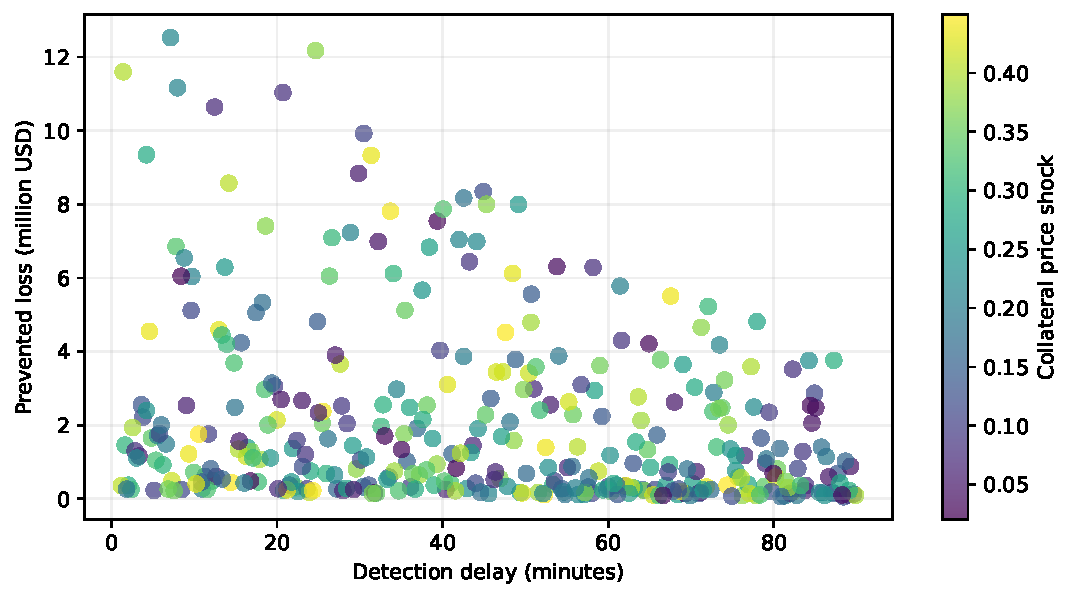
\includegraphics[width=\columnwidth]{../figures/robustness_surface.pdf}
  \caption{MinPause prevented loss across detection delays and collateral price shocks.  Policy coverage remains complete; the economically preventable amount declines with delay.}
  \label{fig:robustness}
\end{figure}

\subsection{Robustness over the sampled space}
MinPause maintains full path coverage in every feasible generated scenario; variation in prevented loss is driven by the potential loss and detection delay rather than by missed paths.  Figure~\ref{fig:robustness} visualizes this distinction.  Long delays leave less loss preventable even when the selected policy is logically sufficient.  Emergency policy synthesis therefore complements, rather than replaces, low-latency monitoring and transaction inclusion.

\section{Discussion}
\subsection{Design implications}
The experiments support three implementation recommendations.  First, protocols should expose distinct pause domains rather than one undifferentiated global flag.  Second, repayment and collateral top-up should be explicitly tested in the paused state; calling them ``allowed'' in documentation is insufficient if a shared internal transfer guard makes them revert.  Third, the action--effect model and candidate policies should be prepared and rehearsed before an incident.  Constructing the model while funds are leaving defeats the latency advantage of a circuit breaker.

MinPause should initially operate in shadow mode.  Given an alert, it can emit a recommended policy and explanation while the guardian retains control.  Historical replay and fork tests should compare the recommendation with known incidents.  Automated execution is only defensible after path-extraction error, false alerts, role compromise, and integration failures are measured.

\subsection{Limitations}
The study is simulation-based and does not claim production deployment or mainnet validation.  Attack paths are supplied rather than automatically discovered.  The reduced-form loss curve, synthetic borrower distribution, and normalized pause costs are controlled experimental assumptions.  Composability can move harm outside the modelled protocol, and a pause transaction can be censored, front-run, or arrive after an atomic exploit.  The solver protects only declared recovery actions and does not prove that external tokens, bridges, or oracles needed by those actions remain live.  Finally, the formal statements in Section~5 require independent completion before the manuscript can claim theoretical guarantees.

\section{Conclusion}
MinPause reframes emergency control as a constrained selection problem rather than an all-or-nothing switch.  Across \ScenarioCount{} reproducible scenarios, it covers all supplied attack paths while preserving \MinAvailability{} of legitimate activity and keeping borrower recovery operations callable.  The result establishes a practical empirical baseline and a transparent artifact.  The next mandatory step is completion and verification of the four formal claims; subsequent work should extract paths from Solidity traces and validate recommendations on historical mainnet forks.

\appendix
\section{Handoff Checklist for Mehran}
The following items are the complete mathematical handoff.  No code changes or empirical reruns are required unless a proof reveals that the model must change.
\begin{enumerate}
  \item Read the definitions in Sections 3 and 4 and normalize notation.
  \item Complete M1, explicitly addressing whether operation sets safely abstract ordered traces.
  \item Prove or correct the iff condition in M2.
  \item Derive exact recovery resource conditions and a finite-reachability statement for M3.
  \item Provide the NP-completeness/NP-hardness reduction requested in M4.
  \item Mark every added assumption and verify that it is respected by the simulation.
  \item Replace each orange box with theorem/proof text only after the claim has been checked.
\end{enumerate}

\section{Artifact Map}
The optimizer is in \texttt{src/minpause/optimizer.py}; scenario generation is in \texttt{src/minpause/scenarios.py}; policy evaluation is in \texttt{src/minpause/simulation.py}; the full run is reproduced by \texttt{scripts/run\_experiments.py}; and tests are in \texttt{tests/}.  Generated CSV files are stored under \texttt{results/} and figures under \texttt{figures/}.

\balance
\bibliographystyle{plain}
\bibliography{references}
\end{document}

